\documentclass[11pt,a4paper]{article}

\usepackage[margin=2.5cm]{geometry}
\usepackage[T1]{fontenc}
\usepackage{lmodern}
\usepackage{microtype}
\usepackage{amsmath,amssymb,bm}
\usepackage{graphicx}
\usepackage{booktabs,longtable,array}
\usepackage{xcolor}
\usepackage{enumitem}
\usepackage[round,authoryear]{natbib}
\usepackage[colorlinks=true,linkcolor=blue!50!black,citecolor=blue!50!black,urlcolor=blue!50!black]{hyperref}
\usepackage[nameinlink,capitalise]{cleveref}

% All numbers below are generated from saved results; regenerate with
%   python scripts/make_report_assets.py      (technical-report assets, shared here)
%   python scripts/make_midproject_assets.py  (mid-project assets)
% Generated by scripts/make_report_assets.py; do not edit.
\newcommand{\NStocksTotal}{500}
\newcommand{\DataStart}{5 January 2010}
\newcommand{\DataEnd}{30 December 2025}
\newcommand{\SplitDate}{1 January 2019}
\newcommand{\InSampleStart}{4 January 2011}
\newcommand{\InSampleDays}{2011}
\newcommand{\SpecN}{467}
\newcommand{\SpecT}{252}
\newcommand{\MPEdge}{5.58}
\newcommand{\NAboveEdge}{8}
\newcommand{\LamOneShare}{36}
\newcommand{\KeptShare}{60}
\newcommand{\EVMean}{57}
\newcommand{\EVMin}{44}
\newcommand{\EVMax}{71}
\newcommand{\EVMaxDate}{June 2012}
\newcommand{\BaseGrossSR}{1.33}
\newcommand{\BaseNetSR}{\ensuremath{-}1.18}
\newcommand{\BaseGrossRet}{4.5}
\newcommand{\BaseNetRet}{\ensuremath{-}4.0}
\newcommand{\BaseVol}{3.4}
\newcommand{\BaseMaxDD}{\ensuremath{-}33.1}
\newcommand{\BaseTurnover}{0.67}
\newcommand{\BaseStockLegTurnover}{0.34}
\newcommand{\BaseHedgeTurnover}{0.33}
\newcommand{\BaseGrossLev}{1.98}
\newcommand{\BaseOpenMean}{156}
\newcommand{\BaseHolding}{9.0}
\newcommand{\BaseBreakeven}{2.6}
\newcommand{\NVariants}{40}

% Generated by scripts/make_midproject_assets.py; do not edit.
\newcommand{\MPNVariants}{40}
\newcommand{\MPNTests}{27}
\newcommand{\MPDeepParams}{1{,}025}
\newcommand{\MPDeepFoldsDone}{3}
\newcommand{\MPBetaBase}{0.024}
\newcommand{\MPCorrBase}{0.11}
\newcommand{\MPBetaBest}{0.035}
\newcommand{\MPCorrBest}{0.14}
\newcommand{\MPBetaETF}{0.037}
\newcommand{\MPBaseCostAnn}{8.4}
\newcommand{\MPBaseGrossAnn}{4.5}
\newcommand{\MPBaseGrossSR}{1.33}
\newcommand{\MPBaseNetSR}{\ensuremath{-}1.18}
\newcommand{\MPBaseBE}{2.6}
\newcommand{\MPBaseLagGrossSR}{0.74}
\newcommand{\MPBaseLagNetSR}{\ensuremath{-}1.75}
\newcommand{\MPBaseLagBE}{1.5}
\newcommand{\MPBestGrossSR}{1.44}
\newcommand{\MPBestNetSR}{0.15}
\newcommand{\MPBestBE}{5.6}
\newcommand{\MPBestLagGrossSR}{1.18}
\newcommand{\MPBestLagNetSR}{\ensuremath{-}0.12}
\newcommand{\MPBestLagBE}{4.5}
\newcommand{\MPETFGrossSR}{1.22}
\newcommand{\MPETFNetSR}{0.02}
\newcommand{\MPETFBE}{5.1}
\newcommand{\MPETFLagGrossSR}{0.82}
\newcommand{\MPETFLagNetSR}{\ensuremath{-}0.39}
\newcommand{\MPETFLagBE}{3.1}
\newcommand{\MPETFStockTO}{0.32}
\newcommand{\MPETFEtfTO}{0.27}
\newcommand{\MPLagLossBase}{44}
\newcommand{\MPLagLossBest}{19}
\newcommand{\MPLagLossETF}{33}


\graphicspath{{figures/}{../figures/}}
\newcommand{\code}[1]{\texttt{#1}}
\DeclareMathOperator{\Var}{Var}
\newcommand{\status}[1]{\textsf{\small #1}}
\setlist{itemsep=2pt,topsep=4pt}

\title{PCA-Based Statistical Arbitrage on US Equities\\[2pt]
\large Mid-Project Report}
\author{Korhan Karadere\\ \small MEng Biomedical Engineering, Imperial College London}
\date{23 October 2026\\ \small Covers work from 13 to 23 October 2026. All results are in-sample (2011--2018);
the 2019--2025 test period has not been evaluated.}

\begin{document}
\maketitle

\begin{abstract}
\noindent This report records the state of an independent project replicating and extending the
PCA statistical arbitrage strategy of \citet{avellaneda2010} on S\&P~500 stocks. A tested
Python implementation, an evaluation protocol with an enforced held-out period, three families
of cost-reduction variants, a sector-ETF factor model, an execution-lag robustness check and a
draft technical report are complete. A deep-learning signal extractor following
\citet{guijarro2021} is implemented and mid-way through walk-forward training. The central
in-sample finding is that the residual mean-reversion signal is statistically strong before
costs (gross Sharpe ratio \MPBaseGrossSR{}) but economically thin: it earns \MPBaseBE{}~bps per
unit traded against an assumed 5~bps cost, giving a net Sharpe ratio of \MPBaseNetSR{}. Reducing
the number of hedged factors and adding a no-trade band raises the break-even cost to
\MPBestBE{}~bps (net Sharpe \MPBestNetSR{}). However, trading one day after the signal instead of
at the signal's own close removes \MPLagLossBest--\MPLagLossBase\% of the gross Sharpe ratio, and
under that realistic timing no variant tested so far is profitable net of costs.
\end{abstract}

\tableofcontents
\newpage

%=====================================================================
\section{Executive summary}
\label{sec:summary}

\begin{table}[ht]
\centering
\caption{Project status at a glance.}
\label{tab:glance}
\small
\begin{tabular}{@{}>{\raggedright\arraybackslash}p{0.43\textwidth}>{\raggedright\arraybackslash}p{0.5\textwidth}@{}}
\toprule
Item & Status \\
\midrule
Core strategy (PCA, OU residuals, s-score, hedging, costs) & Complete, \MPNTests{} automated tests passing at last run \\
Evaluation protocol (in-sample 2011--18 / test 2019--25) & Complete and enforced by tooling; test period unopened \\
Cost-reduction variants (factors, band, frozen hedge, volume) & Complete; \MPNVariants{} distinct configurations evaluated \\
Sector-ETF factor model & Complete \\
Execution-lag robustness check & Complete; materially changes conclusions \\
Technical report (LaTeX, 18 pp.) & First draft complete; results chapter awaits final test \\
Deep-learning extension (CNN+Transformer) & Implemented and tested; training \MPDeepFoldsDone{}/5 yearly folds done (lag 0) \\
Results dashboard & Built for PCA results; deep results pending \\
Version control & Git + private GitHub repository; 4 local commits not yet pushed \\
Statistical tooling (deflated Sharpe, bootstrap) & Not started \\
Per-stock cost model (OHLC spreads) & Not started \\
CRSP survivorship-free data & Not started \\
Final held-out evaluation & Not started; final variants to be pre-registered \\
\bottomrule
\end{tabular}
\end{table}

\paragraph{Key findings to date (in-sample).}
\begin{enumerate}
  \item \textbf{The signal exists.} The Avellaneda--Lee (AL) baseline has a gross Sharpe ratio of
        \MPBaseGrossSR{} with near-zero market beta (\MPBetaBase{}).
  \item \textbf{It does not survive 5~bps costs.} The baseline trades \BaseTurnover{} times its
        capital per day, paying about \MPBaseCostAnn\% a year in costs against \MPBaseGrossAnn\% gross
        return. Net Sharpe is \MPBaseNetSR{}.
  \item \textbf{Hedging is half the cost.} Of the daily turnover, \BaseStockLegTurnover{} is the
        stock leg and \BaseHedgeTurnover{} is hedge trading, mainly baskets traded when positions
        open and close.
  \item \textbf{Fewer factors and a no-trade band double the edge per trade} (break-even
        \MPBaseBE{} $\to$ \MPBestBE{}~bps). The best gross Sharpe occurs at $m=8$ factors, which is also
        the number of correlation eigenvalues above the Marchenko--Pastur noise edge.
  \item \textbf{Execution timing matters most.} Trading at the next close instead of the
        signal's own close cuts gross Sharpe by \MPLagLossBase\% (baseline) and \MPLagLossBest\% (best
        variant). With realistic timing every variant is net-negative at 5~bps.
  \item \textbf{Sector-ETF hedging halves stock turnover} but yields a weaker signal; it is
        approximately break-even at lag~0 (net Sharpe \MPETFNetSR{}).
\end{enumerate}

%=====================================================================
\section{Objectives and scope}
\label{sec:objectives}

The project's aims, fixed at the outset, are:
\begin{enumerate}
  \item Replicate the PCA statistical arbitrage strategy of \citet{avellaneda2010} on a modern
        US large-cap universe with a correct, tested backtest.
  \item Determine whether the strategy is profitable after realistic trading costs and execution
        and, if not, identify precisely where its edge is lost.
  \item Evaluate design changes with an economic rationale (cost reduction, alternative factor
        models, learned signals) under a protocol that prevents overfitting: all design on
        2011--2018, a single final evaluation on 2019--2025.
  \item Deliver a reproducible code base, a technical report whose numbers are generated by the
        code, and a results dashboard.
\end{enumerate}

Out of scope: intraday data, live or paper trading, and any claim about current profitability.

%=====================================================================
\section{Progress against plan}
\label{sec:progress}

The original five-phase roadmap and its status:

\begin{table}[ht]
\centering
\caption{Roadmap status. Dates are completion dates in October 2026.}
\label{tab:roadmap}
\small
\begin{tabular}{@{}p{0.05\textwidth}>{\raggedright\arraybackslash}p{0.45\textwidth}>{\raggedright\arraybackslash}p{0.16\textwidth}>{\raggedright\arraybackslash\footnotesize}p{0.25\textwidth}@{}}
\toprule
Phase & Work package & Status & Evidence \\
\midrule
0 & Baseline replication, data layer, synthetic-data tests & Done (13 Oct) & \code{src/}, \code{tests/} \\
1 & Evaluation protocol; frozen hedges; volume signal; no-trade band; factor-count sweep & Done (14 Oct) & \code{results/sweep\_*} \\
-- & Technical report draft with generated assets & Done (16 Oct) & \code{report/main.pdf} \\
1b & Sector-ETF factor model; execution lag; split stock/ETF costs & Done (20 Oct) & \code{results/etf\_and\_lag} \\
-- & Git, GitHub, relocation off iCloud & Done (20 Oct) & private repository \\
3a & Deep-learning signal extractor & In progress & \code{src/pca\_stat\_arb/deep} \\
2 & Deflated Sharpe, bootstrap CIs, regime analysis & Not started & -- \\
2b & Per-stock spread estimates from OHLC & Not started & -- \\
3b & Marchenko--Pastur adaptive factor count & Not started & -- \\
4 & CRSP/WRDS survivorship-free data & Not started & needs WRDS access \\
5 & Pre-registered held-out evaluation; final report & Not started & -- \\
\bottomrule
\end{tabular}
\end{table}

The order of work changed in one respect. The execution-lag check (originally phase~2) was
brought forward because it could change the project's conclusions, and it did
(\cref{sec:lag}). Statistical tooling was deferred behind the deep-learning extension.

%=====================================================================
\section{System architecture}
\label{sec:arch}

\subsection{Code base}
The implementation is a Python package, \code{pca\_stat\_arb}, built on NumPy, pandas and (for
the deep model) PyTorch. Its structure:

\begin{table}[ht]
\centering
\small
\caption{Modules and responsibilities.}
\label{tab:modules}
\begin{tabular}{@{}l>{\raggedright\arraybackslash}p{0.62\textwidth}@{}}
\toprule
Module & Responsibility \\
\midrule
\code{config} & Typed, immutable configuration from YAML, validated on load \\
\code{data.*} & \code{ReturnsSource} interface; Yahoo Finance loader with parquet cache; universe snapshot; sector-ETF list \\
\code{pca} & Correlation eigendecomposition and eigenportfolio weights \\
\code{residuals} & Batched factor regression, AR(1)/OU fit, s-scores \\
\code{signals} & Three-state trading rule with hysteresis \\
\code{backtest} & Daily walk-forward loop: PCA or ETF factors, daily/frozen hedges, no-trade band \\
\code{accounting} & Shared P\&L engine: execution lag, separate stock/ETF turnover and costs \\
\code{deep.*} & Residual panel, CNN+Transformer model, Sharpe-objective training, yearly walk-forward \\
\code{metrics} & Sharpe, drawdown, turnover, in-sample/test split \\
\code{scripts/experiments.py} & Parallel variant runner; in-sample only unless \code{--reveal-test} \\
\code{scripts/make\_*\_assets.py} & Generate every figure, table and quoted number in the reports \\
\code{scripts/build\_dashboard.py} & Interactive results dashboard with an adjustable cost slider \\
\bottomrule
\end{tabular}
\end{table}

\subsection{Design decisions}
\begin{itemize}
  \item \textbf{One data contract.} All strategies consume a $(\text{dates}\times\text{stocks})$
        table of total returns, so replacing Yahoo Finance with CRSP is confined to one loader.
  \item \textbf{One accounting engine.} Every strategy, including the deep model, is scored by
        the same function, \code{pnl\_from\_holdings} in the \code{accounting} module. Holdings decided at close $t$ are in place from close
        $t+k$ (execution lag $k$) and earn the return of the following day; trades are charged on the
        next day's P\&L. This guarantees that all strategies are compared under identical rules.
  \item \textbf{Vectorised daily step.} One symmetric eigendecomposition, one multi-target
        least-squares solve and closed-form AR(1) estimates per day. A 15-year, 500-stock backtest
        runs in about 45~seconds, which makes sweeps of tens of variants practical.
  \item \textbf{Generated reporting.} Numbers in both reports are \LaTeX{} macros written by
        scripts from saved results, so text cannot drift from code.
\end{itemize}

\subsection{Verification}
The \MPNTests{} automated tests run on a simulated market with known factors and OU residuals.
The most important are the \emph{no-look-ahead} tests. For each strategy family (daily hedges,
frozen hedges with volume adjustment, no-trade band, ETF factors, and the deep model's residual
panel and walk-forward), all data after a cut-off day are replaced with random noise, and the
test asserts that every holding up to that day is unchanged. Other tests check the PCA
spectrum against the Marchenko--Pastur edge, regression orthogonality, recovery of the OU
speed, every transition of the trading rule, per-leg cost accounting, the execution-lag shift,
that the deep model earns nothing on pure noise, and that interrupted training resumes
correctly from checkpoints.

\subsection{Infrastructure}
Code is version-controlled with git and backed up to a private GitHub repository. Licensed or
re-creatable artefacts (price cache, results, Python environment, compiled PDFs, and in future
any CRSP extract) are excluded from version control. The project was moved off the
iCloud-synced Desktop after iCloud interfered with the Python environment
(\cref{sec:issues}).

%=====================================================================
\section{Data}
\label{sec:data}

\begin{itemize}
  \item \textbf{Universe:} the current S\&P~500 list (503 share classes), snapshotted from
        Wikipedia; 500 have Yahoo history.
  \item \textbf{Prices and volume:} daily split- and dividend-adjusted closes and share volume,
        \DataStart{} to \DataEnd{}, from Yahoo Finance via \code{yfinance}. Stored as parquet,
        about 25~MB for $4{,}023 \times 500$ observations of two fields.
  \item \textbf{Sector ETFs:} the nine Select Sector SPDRs trading since 1998 (XLB, XLE, XLF,
        XLI, XLK, XLP, XLU, XLV, XLY), used as factors and hedge instruments in the ETF model.
  \item \textbf{Cleaning:} gaps remain missing (no filled zero returns); zero-volume days are
        treated as non-trading, which removes prices Yahoo backfills before some US listings
        (SW, FERG, AMCR).
\end{itemize}

\paragraph{Known weaknesses.} (i) Survivorship bias: today's constituents applied to 2010--2025.
(ii) No delisting returns. (iii) Only closes and volume are stored, so execution can be
modelled only at closes and costs cannot yet be estimated per stock. (iv) Yahoo adjusted prices
can be revised; the local cache freezes one version.

%=====================================================================
\section{Methodology}
\label{sec:method}

The full derivations are in the technical report. In brief, at each close $t$:

\paragraph{Factors.} Standardised returns over $M=252$ days give a correlation matrix whose top
$m$ eigenvectors $\bm v^{(j)}$ define eigenportfolios with dollar weights
$Q_i^{(j)} = v_i^{(j)}/\sigma_i$ and returns $F_j = \sum_i Q_i^{(j)} R_i$. In the ETF model, the
nine sector-ETF returns replace $F$.

\paragraph{Residuals.} Each stock's last $L=60$ returns are regressed on the factors,
$R_i = \alpha_i + \sum_j \beta_{ij} F_j + \varepsilon_i$. The cumulative residual
$X_i = \sum \varepsilon_i$ is fitted as an AR(1), $X_{k+1} = a + bX_k + \zeta$, and mapped to OU
parameters $\kappa = -252\ln b$, $m = a/(1-b)$, $\sigma_{\text{eq}} = \sqrt{\Var(\zeta)/(1-b^2)}$.
Stocks with $\kappa < 252/30$ are ineligible.

\paragraph{Signal and positions.} The s-score $s_i = -\tilde m_i / \sigma_{\text{eq},i}$
(cross-sectionally centred $m$) drives a three-state rule: open long at $s<-1.25$, open short
at $s>1.25$, close longs at $s>-0.50$ and shorts at $s<0.75$. Each open position of
$q = 1\%$ of capital is hedged by the factors; in stock space the book is
$\bm w^{\text{net}} = \bm w - Q B^\top \bm w$. In the ETF model the hedge is held directly as
$-B^\top \bm w$ dollars of the ETFs.

\paragraph{Variants.} \emph{Frozen hedges} fix each position's hedge at entry. The \emph{volume
signal} scales returns by $\langle V\rangle_{10}/V_t$ before the residual fit. The \emph{no-trade
band} leaves a holding unchanged if the required trade is below $\delta$. \emph{Execution lag}
$k$ delays all holdings by $k$ days.

\paragraph{Accounting.} Daily P\&L is
$\text{net}_{t+1} = \bm w_t^\top \bm R_{t+1} - c_s\|\Delta \bm w^{\text{stock}}_t\|_1 - c_e\|\Delta \bm w^{\text{ETF}}_t\|_1$
with $c_s = 5$~bps and $c_e = 1$~bp one-way, on fixed capital. The break-even stock cost is
$c^\ast = (\overline{\text{gross}} - c_e\,\overline{\text{TO}}_{\text{ETF}})/\overline{\text{TO}}_{\text{stock}}$.

%=====================================================================
\section{Results to date (in-sample, 2011--2018)}
\label{sec:results}

\subsection{Factor structure}
On the last in-sample day, \NAboveEdge{} eigenvalues of the \SpecN-stock correlation matrix
exceed the Marchenko--Pastur edge of \MPEdge{} (\cref{fig:spectrum}). The 15 baseline factors
explain on average \EVMean\% of variance.

\begin{figure}[ht]
\centering
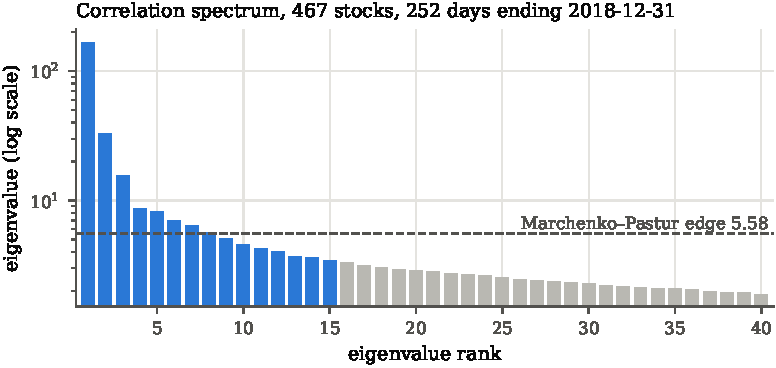
\includegraphics[width=\textwidth]{spectrum}
\caption{Leading eigenvalues of the 252-day correlation matrix ending 31 December 2018, with the
Marchenko--Pastur noise edge. Blue: the 15 baseline factors.}
\label{fig:spectrum}
\end{figure}

\subsection{Baseline and cost decomposition}
The AL baseline earns a gross Sharpe ratio of \MPBaseGrossSR{} but \MPBaseNetSR{} net of costs
(\cref{fig:cumpnl}). Its market beta, estimated against the equal-weighted universe, is
\MPBetaBase{} (correlation \MPCorrBase{}), so the hedging achieves market neutrality. Turnover is
split almost equally between the stock leg (\BaseStockLegTurnover) and hedges
(\BaseHedgeTurnover). Frozen hedges reduce turnover only slightly (0.67 $\to$ 0.61), which shows
that the hedge cost arises mainly when positions open and close, not from daily re-hedging.

\begin{figure}[ht]
\centering
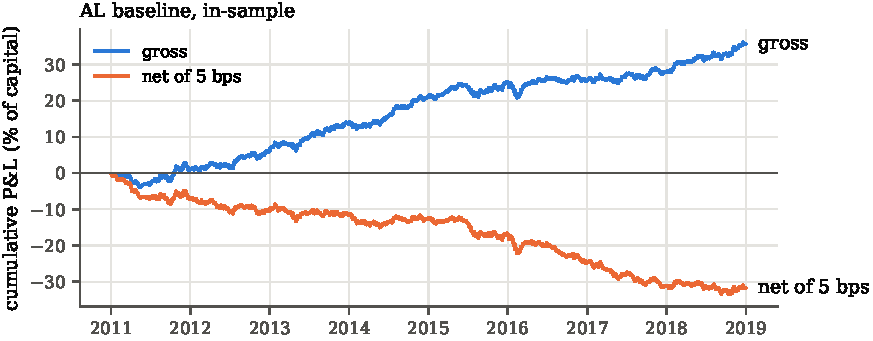
\includegraphics[width=\textwidth]{cum_pnl_baseline}
\caption{Cumulative in-sample P\&L of the AL baseline, gross and net of 5~bps (lag 0).}
\label{fig:cumpnl}
\end{figure}

\subsection{Number of factors and no-trade band}
Gross Sharpe rises with the number of factors up to $m=8$ and then falls, while turnover rises
monotonically because every factor adds a basket across the whole universe
(\cref{fig:tradeoff}). Combining $m=8$ with a no-trade band $\delta = 0.002$ gives the best
in-sample break-even cost, \MPBestBE{}~bps (gross Sharpe \MPBestGrossSR, net \MPBestNetSR).
Wider entry thresholds reduce turnover but lower the break-even cost, so extreme s-scores are not
more profitable per unit traded. The volume adjustment did not help in this period.

\begin{figure}[ht]
\centering
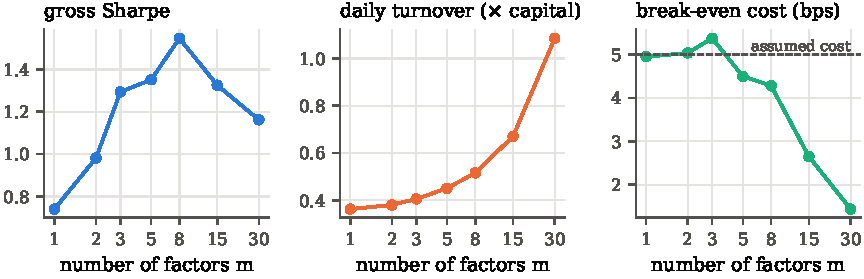
\includegraphics[width=\textwidth]{factor_tradeoff}
\caption{Gross Sharpe, turnover and break-even cost against the number of hedged factors.}
\label{fig:tradeoff}
\end{figure}

\subsection{Execution lag and sector ETFs}
\label{sec:lag}
\Cref{tab:lag} reports the main variants with and without a one-day execution lag. Trading at the
close that produced the signal is AL's convention, but it is not achievable in practice. It also
benefits from bid--ask bounce: a closing price that happens to print at the bid or ask produces an
apparent reversal that the strategy then ``captures''. With the lag, gross Sharpe falls by
\MPLagLossBase\% for the baseline, \MPLagLossBest\% for the best variant and \MPLagLossETF\% for the ETF model
(\cref{fig:lag}). Every variant becomes net-negative at 5~bps.

\begin{table}[ht]
\centering
\caption{In-sample results with execution lag 0 and 1 (5~bps stock cost; 1~bp ETF cost unless
noted). TO: mean daily one-way turnover ($\times$ capital). BE: break-even stock cost.}
\label{tab:lag}
\small
\setlength{\tabcolsep}{4pt}
\begin{tabular}{@{}lrrrrrrr@{}}
\toprule
Variant & Gross SR & Net SR & Net ret. & Max DD & TO$_{\text{stock}}$ & TO$_{\text{ETF}}$ & BE (bps)\\
\midrule
AL baseline ($m=15$) & 1.33 & \ensuremath{-}1.18 & \ensuremath{-}4.0\% & \ensuremath{-}33.1\% & 0.67 & 0.00 & 2.6\\
\quad lag 1 & 0.74 & \ensuremath{-}1.75 & \ensuremath{-}5.9\% & \ensuremath{-}48.2\% & 0.67 & 0.00 & 1.5\\
\midrule
$m=8$, $\delta=0.002$ & 1.44 & 0.15 & 0.6\% & \ensuremath{-}7.5\% & 0.37 & 0.00 & 5.6\\
\quad lag 1 & 1.18 & \ensuremath{-}0.12 & \ensuremath{-}0.4\% & \ensuremath{-}11.1\% & 0.37 & 0.00 & 4.5\\
\midrule
$m=3$, $\delta=0.0005$ & 1.24 & 0.17 & 0.7\% & \ensuremath{-}7.6\% & 0.36 & 0.00 & 5.8\\
\quad lag 1 & 0.97 & \ensuremath{-}0.12 & \ensuremath{-}0.5\% & \ensuremath{-}12.4\% & 0.36 & 0.00 & 4.5\\
\midrule
Sector ETFs (1 bp hedges) & 1.22 & 0.02 & 0.1\% & \ensuremath{-}10.9\% & 0.32 & 0.27 & 5.1\\
\quad lag 1 & 0.82 & \ensuremath{-}0.39 & \ensuremath{-}1.5\% & \ensuremath{-}20.5\% & 0.32 & 0.27 & 3.1\\
\quad ETF cost 2 bps & 1.22 & \ensuremath{-}0.15 & \ensuremath{-}0.6\% & \ensuremath{-}13.1\% & 0.32 & 0.27 & 4.3\\
\bottomrule
\end{tabular}

\end{table}

\begin{figure}[ht]
\centering
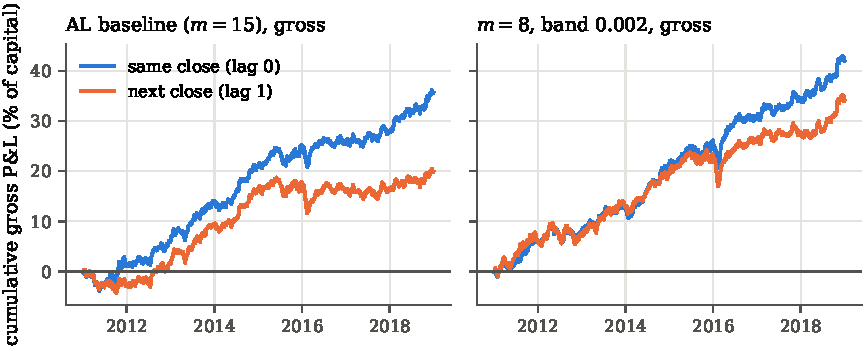
\includegraphics[width=\textwidth]{lag_gross}
\caption{Cumulative gross P\&L with trading at the signal's close (lag 0) and at the next close
(lag 1).}
\label{fig:lag}
\end{figure}

The sector-ETF model halves stock turnover (\MPETFStockTO{} per day, plus \MPETFEtfTO{} of cheap
ETF trading), but its residuals carry a weaker signal (gross Sharpe \MPETFGrossSR{} versus
\MPBaseGrossSR{}). Netting the book's hedge into nine ETF positions is effective; what is lost is
the quality of the residual.

\subsection{Cost sensitivity}
Because the conclusion hinges on the cost assumption, \cref{fig:costs} shows net Sharpe as a
function of the stock cost, computed from the saved gross P\&L and turnover. At lag~0 the best
variants break even at about 5--6~bps. At lag~1 they need costs below about 4.5~bps, a level
achievable for large institutions trading S\&P~500 names but not established for this
strategy. A per-stock cost model is therefore needed before drawing a final conclusion.

\begin{figure}[ht]
\centering
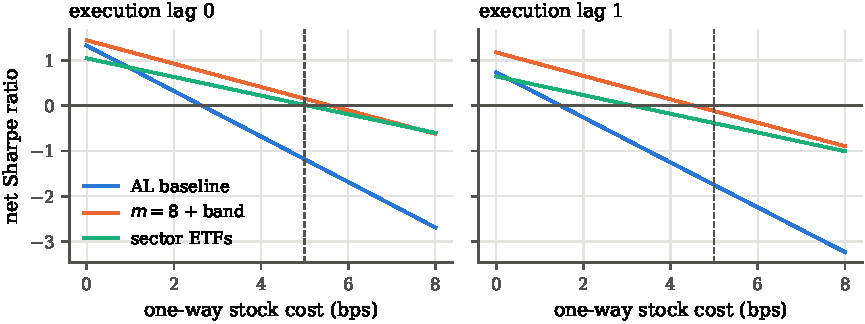
\includegraphics[width=\textwidth]{cost_sensitivity}
\caption{Net Sharpe ratio against one-way stock cost (ETF leg fixed at 1~bp), in-sample.
Dashed line: the assumed 5~bps.}
\label{fig:costs}
\end{figure}

%=====================================================================
\section{Deep-learning extension (in progress)}
\label{sec:deep}

\subsection{Motivation}
The AL rule uses a parametric model (OU) and fixed thresholds. \citet{guijarro2021} replace both
with a neural network that maps each stock's recent residual path to a position, trained to
maximise the net Sharpe ratio directly. This tests whether a flexible signal extractor can find
a profitable pattern in the same residuals that the OU rule cannot exploit after costs.

\subsection{Design}
\paragraph{Out-of-sample residuals.} At each close $t$ an 8-factor PCA model (the
Marchenko--Pastur count found in-sample) is fitted on data up to $t$. The residual of day $t+1$
uses only those already-known loadings:
\[
  \varepsilon_{t+1} = R_{t+1} - B_t\left(Q_t^\top R_{t+1}\right).
\]
A residual position $\bm w$ is a genuine stock portfolio,
$\bm w^{\text{stock}} = \bm w - Q_t B_t^\top \bm w$, which earns exactly
$\bm w^\top \varepsilon_{t+1}$, a property verified by a test. The network is therefore trained
on residual returns while costs are charged on the implied stock trades.

\paragraph{Inputs.} For each stock, the cumulative residual path over the last 30 days, divided by
the cross-sectional standard deviation of all paths that day.

\paragraph{Architecture.} Two 1-D convolutional blocks (8 filters, kernel 2, instance
normalisation, residual connections) extract local shape features. A learned positional
embedding and one Transformer encoder layer (4 heads, model width 8, feed-forward width 16,
dropout 0.25) relate every point of the path to every other. A linear head on the final time
step outputs one score per stock. The model has \MPDeepParams{} parameters.

\paragraph{Allocation and objective.} Scores are normalised to unit gross exposure each day,
$w_i = f_i/\sum_k |f_k|$. Training maximises the annualised Sharpe ratio of daily net returns,
$-\sqrt{252}\,\overline{r}/\operatorname{sd}(r)$ with
$r_{t+1} = \bm w_t^\top \varepsilon_{t+1+k} - c_s\|\Delta\bm w^{\text{stock}}_t\|_1$, computed over
63-day blocks with half-overlapping starts. Adam (learning rate $10^{-3}$), up to 60 epochs, and
early stopping with patience 10 on the validation net Sharpe. The model is trained for the
execution lag $k$ it will be deployed with.

\paragraph{Walk-forward protocol.} For each trading year $y \in \{2014,\dots,2018\}$, the model is
trained on all data from 15 February 2011 (the first day with complete features) to the end of
$y-2$, validated on year $y-1$, and then trades year $y$ frozen. Training stops $1+k$ days before
the trading year so that no label overlaps it. Three seeds are trained per year and their scores
averaged. All hyper-parameters are fixed in advance from the paper, so the model counts as one
trial per lag, not a search. The data are truncated at the split date, so 2019--2025 is never
seen.

\paragraph{Engineering.} Training runs on the Apple-silicon GPU (PyTorch MPS). The first attempt
used about 15~GB of unified memory and made the machine unusable. Memory was cut below 4~GB by
scoring validation and trading days in 21-day chunks, training on 63-day blocks, capping the
MPS allocator and releasing its cache after every step. An earlier lag-1 attempt hit the
allocator cap and stopped; the cap was raised and the launcher now stops on failure. Finished
years are checkpointed, so an interrupted run resumes.

\subsection{Status}
At the time of writing (23 October, 23:00), the lag-0 run has completed \MPDeepFoldsDone{} of its
five yearly folds and is training the 2017 fold; the lag-1 run follows. \Cref{tab:folds} lists the best validation Sharpe of each ensemble member.

\begin{table}[ht]
\centering
\caption{Completed walk-forward folds (lag 0): best validation net Sharpe per seed. These are
maxima over epochs and therefore optimistic; they are not trading results.}
\label{tab:folds}
\small
\begin{tabular}{@{}llllrrr@{}}
\toprule
Trade year & Train from & Train to & Validate on & Seed 0 & Seed 1 & Seed 2\\
\midrule
2014 & 2011-02-15 & 2012-12-31 & 2013 & 1.71 & 0.10 & 1.61\\
2015 & 2011-02-15 & 2013-12-31 & 2014 & 1.41 & 1.32 & 1.26\\
2016 & 2011-02-15 & 2014-12-31 & 2015 & \ensuremath{-}0.91 & \ensuremath{-}0.75 & \ensuremath{-}0.55\\
\bottomrule
\end{tabular}

\end{table}

Early observations, which are provisional:
\begin{itemize}
  \item Validation scores for the 2014 and 2015 folds are positive net of 5~bps, but one seed in
        2014 (0.10) differs sharply from the others (1.71, 1.61). Training is seed-sensitive,
        which supports ensembling.
  \item In the 2016 fold (validated on 2015), all three seeds have negative best validation
        scores ($-0.91$, $-0.75$, $-0.55$): on 2015 the model found no configuration that is
        profitable net of costs. This is the same cost barrier the PCA rule faces.
  \item Trading-year results will be reported only after all folds finish, against the AL
        baseline over the same years. The tuned PCA variants were selected using data that
        includes 2014--2018, so comparing against them would flatter the PCA side.
\end{itemize}

%=====================================================================
\section{Issues encountered and resolutions}
\label{sec:issues}

\begin{table}[ht]
\centering
\caption{Problems met so far and how they were resolved.}
\label{tab:issues}
\small
\begin{tabular}{@{}>{\raggedright\arraybackslash}p{0.3\textwidth}>{\raggedright\arraybackslash}p{0.32\textwidth}>{\raggedright\arraybackslash}p{0.3\textwidth}@{}}
\toprule
Issue & Cause & Resolution \\
\midrule
Python imports failed & iCloud set a hidden flag on a \code{.pth} file; Python 3.13 skips hidden \code{.pth} files & Project moved to \code{\textasciitilde/Projects}; flag cleared; tests set \code{pythonpath} \\
Corrupted ETF cache & Parallel workers downloaded and read the same file concurrently & Atomic write-then-rename; cache filled before workers start \\
Report mislabelled a variant & Asset script read a fixed list of configs & Reads all configs; unknown variants raise an error \\
Deep training used 15~GB & Full-period tensors on GPU & Chunked evaluation, block training, allocator cap, cache release \\
Lag-1 training stopped & MPS out-of-memory at the 4.4~GB cap & Cap raised; launcher stops and resumes cleanly \\
git and Homebrew unavailable & Xcode licence not accepted & Licence accepted; Tectonic installed from release binary \\
Synthetic tests too strict & Weak simulated factors made beta estimates noisy & Exact algebraic checks plus statistical checks on the dominant factor \\
\bottomrule
\end{tabular}
\end{table}

%=====================================================================
\section{Risks and limitations}
\label{sec:risks}

\begin{enumerate}
  \item \textbf{Survivorship bias} may flatter or distort results; CRSP is the remedy (needs a
        WRDS account).
  \item \textbf{Cost model.} A flat 5~bps for every stock decides the sign of the result. Without
        per-stock estimates, the conclusion ``not profitable'' is conditional on this
        assumption.
  \item \textbf{Multiple testing.} \MPNVariants{} PCA/ETF configurations plus the deep model at two
        lags have been evaluated in-sample. Best-of-many Sharpe ratios must be deflated
        \citep{bailey2014}.
  \item \textbf{Execution model.} Only close prices are available; next-open execution and
        intraday timing cannot be tested yet.
  \item \textbf{Deep model risk.} Seed sensitivity and early negative validation scores suggest
        that it may not beat the cost barrier either; it must be judged on trading years only.
  \item \textbf{Unpushed work.} Four commits exist only locally; they should be pushed to GitHub.
\end{enumerate}

%=====================================================================
\section{Plan for the remaining work}
\label{sec:plan}

In order of priority:
\begin{enumerate}
  \item \textbf{Finish deep training} (lag 0 and lag 1) and report trading-year results against the
        AL baseline over 2014--2018, with figures and the dashboard update.
  \item \textbf{Per-stock cost model:} store open, high and low prices; estimate spreads
        (e.g.\ Corwin--Schultz); re-evaluate the shortlisted variants. Add next-open execution.
  \item \textbf{Statistical tooling:} deflated Sharpe ratio using the full trial count, block
        bootstrap confidence intervals, and performance by regime.
  \item \textbf{Adaptive factor count:} choose $m_t$ daily as the number of eigenvalues above the
        Marchenko--Pastur edge. This is the main original contribution.
  \item \textbf{Pre-register} the final variants (AL baseline; best PCA variant; ETF model; deep
        model; adaptive-$m$), all at lag 1, then run the 2019--2025 test \emph{once}.
  \item \textbf{CRSP} replication if WRDS access is granted, then finalise the technical report.
\end{enumerate}

The project's conclusion will be reported whichever way the held-out test falls. A rigorously
diagnosed negative result (that a well-known strategy no longer survives realistic costs and
execution, and why) is a valid and useful outcome.

\bibliographystyle{plainnat}
\bibliography{../references}

\appendix
\section{All evaluated PCA and ETF variants}
\label{app:variants}
In-sample statistics of all \MPNVariants{} distinct configurations (including the execution-lag
and sector-ETF runs), sorted by net Sharpe. Overrides are relative to the AL baseline. Columns:
gross and net Sharpe, annualised net volatility, mean daily turnover (stock plus ETF) and
break-even stock cost.

{\small
\begin{longtable}{@{}l>{\raggedright\arraybackslash\footnotesize}p{4.4cm}rrrrr@{}}
\toprule
Variant & Overrides & Gross SR & Net SR & Vol & Turnover & BE (bps)\\
\midrule
\endhead
\texttt{f3\_band05} & \texttt{n\_factors=3, rebalance\_band=0.0005} & 1.24 & 0.17 & 4.2\% & 0.36 & 5.8\\
\texttt{f8\_band20} & \texttt{n\_factors=8, rebalance\_band=0.002} & 1.44 & 0.15 & 3.6\% & 0.37 & 5.6\\
\texttt{f3\_band10} & \texttt{n\_factors=3, rebalance\_band=0.001} & 1.14 & 0.14 & 4.3\% & 0.34 & 5.7\\
\texttt{f1\_exitneg} & \texttt{n\_factors=1, s\_open=2.0, s\_close\_long=\ensuremath{-}0.5, s\_close\_short=\ensuremath{-}0.5} & 0.48 & 0.13 & 4.1\% & 0.11 & 6.9\\
\texttt{f3} & \texttt{n\_factors=3} & 1.29 & 0.09 & 4.2\% & 0.41 & 5.4\\
\texttt{f3\_frozen} & \texttt{n\_factors=3, hedge\_mode=frozen} & 1.21 & 0.05 & 4.3\% & 0.40 & 5.2\\
\texttt{f8\_band10} & \texttt{n\_factors=8, rebalance\_band=0.001} & 1.51 & 0.03 & 3.6\% & 0.42 & 5.1\\
\texttt{f2} & \texttt{n\_factors=2} & 0.98 & 0.01 & 4.9\% & 0.38 & 5.0\\
\texttt{f1} & \texttt{n\_factors=1} & 0.74 & \ensuremath{-}0.01 & 6.1\% & 0.36 & 4.9\\
\texttt{f5\_exitneg} & \texttt{n\_factors=5, s\_open=2.0, s\_close\_long=\ensuremath{-}0.5, s\_close\_short=\ensuremath{-}0.5} & 0.75 & \ensuremath{-}0.04 & 2.7\% & 0.17 & 4.7\\
\texttt{f5\_frozen} & \texttt{n\_factors=5, hedge\_mode=frozen} & 1.33 & \ensuremath{-}0.10 & 3.9\% & 0.44 & 4.7\\
\texttt{f3\_exitneg} & \texttt{n\_factors=3, s\_open=2.0, s\_close\_long=\ensuremath{-}0.5, s\_close\_short=\ensuremath{-}0.5} & 0.48 & \ensuremath{-}0.13 & 2.9\% & 0.14 & 3.9\\
\texttt{f8\_band05} & \texttt{n\_factors=8, rebalance\_band=0.0005} & 1.51 & \ensuremath{-}0.14 & 3.6\% & 0.47 & 4.6\\
\texttt{f5} & \texttt{n\_factors=5} & 1.35 & \ensuremath{-}0.15 & 3.8\% & 0.45 & 4.5\\
\texttt{f8} & \texttt{n\_factors=8} & 1.55 & \ensuremath{-}0.26 & 3.6\% & 0.52 & 4.3\\
\texttt{open200\_close\_neg} & \texttt{s\_open=2.0, s\_close\_long=\ensuremath{-}0.5, s\_close\_short=\ensuremath{-}0.5} & 1.00 & \ensuremath{-}0.53 & 2.6\% & 0.31 & 3.3\\
\texttt{f15\_band20} & \texttt{rebalance\_band=0.002} & 1.26 & \ensuremath{-}0.54 & 3.4\% & 0.49 & 3.5\\
\texttt{f15\_band10} & \texttt{rebalance\_band=0.001} & 1.30 & \ensuremath{-}0.85 & 3.4\% & 0.58 & 3.0\\
\texttt{open125\_close0} & \texttt{s\_close\_long=0.0, s\_close\_short=0.0} & 1.14 & \ensuremath{-}0.88 & 4.1\% & 0.65 & 2.8\\
\texttt{open200\_close0} & \texttt{s\_open=2.0, s\_close\_long=0.0, s\_close\_short=0.0} & 0.82 & \ensuremath{-}0.88 & 2.2\% & 0.30 & 2.4\\
\texttt{f15\_band05} & \texttt{rebalance\_band=0.0005} & 1.32 & \ensuremath{-}1.05 & 3.4\% & 0.63 & 2.8\\
\texttt{frozen\_hedge} & \texttt{hedge\_mode=frozen} & 1.16 & \ensuremath{-}1.10 & 3.4\% & 0.61 & 2.6\\
\texttt{resid90} & \texttt{residual\_window=90} & 0.91 & \ensuremath{-}1.10 & 3.1\% & 0.49 & 2.3\\
\texttt{slow\_ok\_kappa} & \texttt{kappa\_min=4.2} & 1.28 & \ensuremath{-}1.11 & 3.5\% & 0.65 & 2.7\\
\texttt{open200} & \texttt{s\_open=2.0} & 0.83 & \ensuremath{-}1.14 & 1.8\% & 0.28 & 2.1\\
\texttt{volume\_signal} & \texttt{volume\_adjust=True} & 1.29 & \ensuremath{-}1.15 & 3.3\% & 0.63 & 2.6\\
\texttt{baseline} & \texttt{--} & 1.33 & \ensuremath{-}1.18 & 3.4\% & 0.67 & 2.6\\
\texttt{open150} & \texttt{s\_open=1.5} & 1.11 & \ensuremath{-}1.21 & 2.9\% & 0.54 & 2.4\\
\texttt{frozen\_volume} & \texttt{hedge\_mode=frozen, volume\_adjust=True} & 1.01 & \ensuremath{-}1.21 & 3.3\% & 0.59 & 2.3\\
\texttt{open175} & \texttt{s\_open=1.75} & 0.86 & \ensuremath{-}1.33 & 2.3\% & 0.40 & 2.0\\
\texttt{fast\_kappa} & \texttt{kappa\_min=16.8} & 1.36 & \ensuremath{-}1.64 & 2.9\% & 0.69 & 2.3\\
\texttt{factors30} & \texttt{n\_factors=30} & 1.16 & \ensuremath{-}2.87 & 3.4\% & 1.09 & 1.4\\
\bottomrule
\end{longtable}

}

\end{document}
